\documentclass[runningheads,a4paper]{llncs}

\usepackage{amssymb}
\usepackage{amsmath}
\usepackage{subfig}

\usepackage{graphicx}
\usepackage{cite}
\usepackage{url}
\urldef{\mails}\path|{yang.deng, zhonghong.ou, antti.yla-jaaski}@aalto.fi|
\newcommand{\keywords}[1]{\par\addvspace\baselineskip
\noindent\keywordname\enspace\ignorespaces#1}

\begin{document}

\mainmatter

\title{Adaptive Packet Size Control for \\Bulk Data Transmission in IPv6 over \\Networks of Resource Constrained Nodes}
\titlerunning{Adaptive Packet Size Control for Bulk Data Transmission in 6lo}

\author{Yang Deng\and Zhonghong Ou\and Antti Yl\"a-J\"a\"aski}
\authorrunning{Y.Deng et al.}

\institute{Aalto University, Espoo, Finland\\ \mails}

\maketitle

\begin{abstract}
Conventional transmission in IPv6 over Networks of Resource Constrained Nodes~(6lo) favours fixed-size packets and results in low network performance when bulk data transmission is required by applications, for example firmware updating. To tackle this problem, we first investigate performance of bulk data transmission through large packets and make two important observations. Then we propose an adaptive mechanism at IP layer to dynamically adjust packet size in 6lo. We implemented the mechanism on Contiki OS and evaluated it through a series of experiments in Cooja. Experimental results demonstrate that our mechanism outperforms Contiki standard implementation significantly from both reliability and goodput under various network conditions.

\keywords{6lo, Bulk Data Transmission, Packet Size Control}
\end{abstract}

\section{Introduction}
IPv6 over Networks of Resource-constrained Nodes~(6lo) is a network that provides IPv6 connectivity over constrained nodes such as sensors or actuators. It introduces an adaptation layer to deal with the mapping between IPv6 packets and link frames (hereafter referred to as \texttt{packet} and \texttt{frame} respectively). Conventionally, when data are transmitted in 6lo, they are firstly encapsulated into a fixed-size packet and then header compression is applied to reduce the packet size. If the compressed packet fits into a single frame then it will be sent out instantly; otherwise fragmentation-reassembly mechanism (hereafter referred to as \texttt{6lo fragmentation}) is invoked. The value of the fixed-size is preconfigured empirically (e.g. 140 bytes for IEEE 802.15.4 in Contiki). As RFC4944~\cite{Rfc4944} points out, in links with a small maximum transmission unit (MTU), the conventional transmission works but with two assumptions: (i) most applications will not use large packets and (ii) application payload is relatively small. Nevertheless, there are application scenarios where these conditions do not hold. Considering firmware updating on-the-fly or massive data exchanging between nodes, both of them involve bulk data transmission for which 6lo conventional transmission is not suitable due to low network performance.

In order to improve 6lo performance of bulk data transmission, we present an adaptive mechanism that adjusts packet size dynamically based on network conditions and utilizes 6lo fragmentation (different from IP fragmentation) to send large packets. Unlike other adaptive mechanisms~\cite{Dong2010, Jele2008, Ou2009}, our mechanism works at IP layer whereas others only work at link layer. Link layer mechanisms highly rely on the link of a specific type. For example the mechanism designed for IEEE 802.15.4 might not be feasible for Bluetooth Low Energy (BLE) or Near Field Communication (NFC), both are documented by 6lo working group. As 6lo operates over links of different types, an upper-layer mechanism is therefore much more desirable. Furthermore, even if frame size can be dynamically controlled by link layer mechanisms, there remains a need for determining IP packet size in 6lo. Unfortunately, to the best of our knowledge, such a mechanism is still missing so far. Our work fills in this gap and in summary it makes three key contributions as follows:
\begin{itemize}
\item We investigate performance of bulk data transmission in 6lo through large packets and make two important observations.
\item We present design, implementation, and evaluation of IP layer adaptive mechanism suitable for bulk data transmission in 6lo.
\item We demonstrate that our adaptive mechanism is able to provide better reliability and higher goodput than Contiki standard implementation under various network conditions.
\end{itemize}

\section{Related Work}
Before IPv6 is introduced to Wireless Sensor Network (WSN), frame size optimization for WSN has been studied extensively in literature. Modiano~et~al.~\cite{Modi1999} developed a Markov chain model to analyse the channel then performed a maximum likelihood approach to estimate frame size. Sankarasubramaniam~et~al.~\cite{Sank2003} used energy-efficiency as the optimization object to determine the best frame size based on a set of radio and channel parameters. The work from~\cite{Vura2008} discussed the cross-layer solutions to set frame size for different environments like underwater and underground networks. All of these studies focus on finding an optimal fixed size. Another thread of research work suggests using adaptive approaches. Jelenkovi\'{c}~et~al.~\cite{Jele2008} designed an algorithm to divide the frame into several small chunks to fit available channel periods. Dong's work~\cite{Dong2010} followed a similar idea that small chunks can be reassembled into a bigger frame. Nonetheless, these solutions work only at link layer. Because 6lo has a wide diversity of links, a solution working at IP layer is beneficial, which is the main contribution of this paper.

\section{Mechanism}

\subsection{Overview}\label{sec:ov}
Our motivation comes from the assumption (justified in section~\ref{sec:vd}) that bulk data transmission in 6lo by using large packets (invoking 6lo fragmentation if necessary) can improve network performance significantly. Nodes in 6lo usually suffer from intra-path interference~\cite{Kim2007}, which means that when the successor node forwards the packet at the same time it will prevent the reception of following packet coming from the predecessor node. Employing pipeline mechanisms to send packets might mitigate this problem; however, a poorly-designed scheduling policy can cause traffic congestion and lead to an even worse situation. Thus, stop-and-wait Automatic Repeat reQuest (ARQ) is the widely-used protocol to transmit bulk data in 6lo. One good example is Contiki TCP implementation where the window size is~1. In stop-and-wait ARQ, transmission time decreases as packet size increases. Nonetheless, the desire for large packets is limited by network conditions because the whole packet has to be retransmitted if any of the fragments gets lost. To tackle this problem, we propose an adaptive mechanism to adjust packet size based on network conditions; if network condition becomes better the packet size is increased, otherwise it is decreased.

For simplicity and practicality, network conditions are indicated by packet loss rate (PLR)~\cite{Bacc2012}. Through empirical experiments, we make two important \textbf{observations}: (1) PLR of large packets is mainly impacted by the number of fragments that the packet is divided into; (2) if frame length is relatively small (approximately 100 octets), it has a trivial influence on the PLR. Due to space limit, we omit the analysis here. Inspired by these two observations, we propose an adaptive mechanism by following two rules:
\begin{description}
	\item[Rule 1.] Adjust packet size by fragments rather than octets, which is deduced from observation (1).
	\item[Rule 2.] Given the number of fragments, make sure each fragment fills the frame as fully as possible, which is deduced from observation (2).
\end{description}
Based on these two rules, we design two modules, i.e., \emph{Unit Discovery Module} and \emph{Packet Adjustment Module}, to enable the adaptive mechanism.

\subsection{Unit Discovery Module}
\emph{Unit Discovery Module} is responsible for finding the unit value by which packet size is increased/decreased in the mechanism. Considering a multi-hop 6lo, the unit value should be the \emph{maximum} size of packet that will not be fragmented by any node along the path from the sender to the receiver. Note that given a packet, the decision on whether it should be fragmented or not is different at different nodes along the path. For example, by default 6lo employs Routing Protocol for Low power and Lossy Networks (RPL) as its routing protocol, the intermediate nodes between the sender and the receiver might insert RPL options into the packet. As a consequence, the packet without need of fragmentation at the sender might be fragmented at an intermediate router. To tackle this problem, we introduce a discovery procedure similar to Path MTU Discovery (PMTUD). Before bulk data transmission starts, the sender pings the receiver using an Internet Control Message Protocol (ICMP) Echo Request message whose size is the current unit value. After an intermediate node receives this message it checks whether 6lo fragmentation is needed or not. If yes, the node drops the message and sends back an ICMP Packet Too Big message containing the new appropriate unit value to the sender. Upon receiving ICMP Packet Too Big message, the sender re-pings the receiver by a new ICMP Echo Request message whose size is the updated unit value. The discovery procedure continues until the sender receives an ICMP Echo Reply message from the target receiver. The unit value corresponding to the receiver is saved in a cache and ready for use in \emph{Packet Adjustment Module}.

\subsection{Packet Adjustment Module} \label{sec:pa}
Once the unit value is discovered, \emph{Packet Adjustment Module} uses it to adjust packet size according to network conditions, assuming that the routing information is not changed throughout the course of bulk data transmission. Packet size is adjusted by the following equation (note that 6lo fragmentation cuts the packets into 8-octet units):
\begin{equation} \label{eq:size}
S(n) = \left\{
  \begin{array}{c l}
    U & \quad n=1 \\
    \lfloor \frac{U-L_{F1}}{8} \rfloor \times 8 + \lfloor \frac{M-L_{FN}}{8} \rfloor \times 8 \times (n-2) + (M-L_{FN}) & \quad n \ge 2
  \end{array}
\right.
\end{equation}
where $U$ is the unit value and $M$ is the link MTU, $L_{F1}$ and $L_{FN}$ (4 and 5 in 6lo) are the length of initial fragment header and non-initial fragment header. It is important to note here that $n$ should be less than $10$ as (i) PLR increases significantly as $n$ grows, and (ii) constrained nodes do not have enough memory to collect many fragments.

\begin{figure}
	\vspace{-15pt}
	\centering
	\subfloat[Negative exponential relationship]{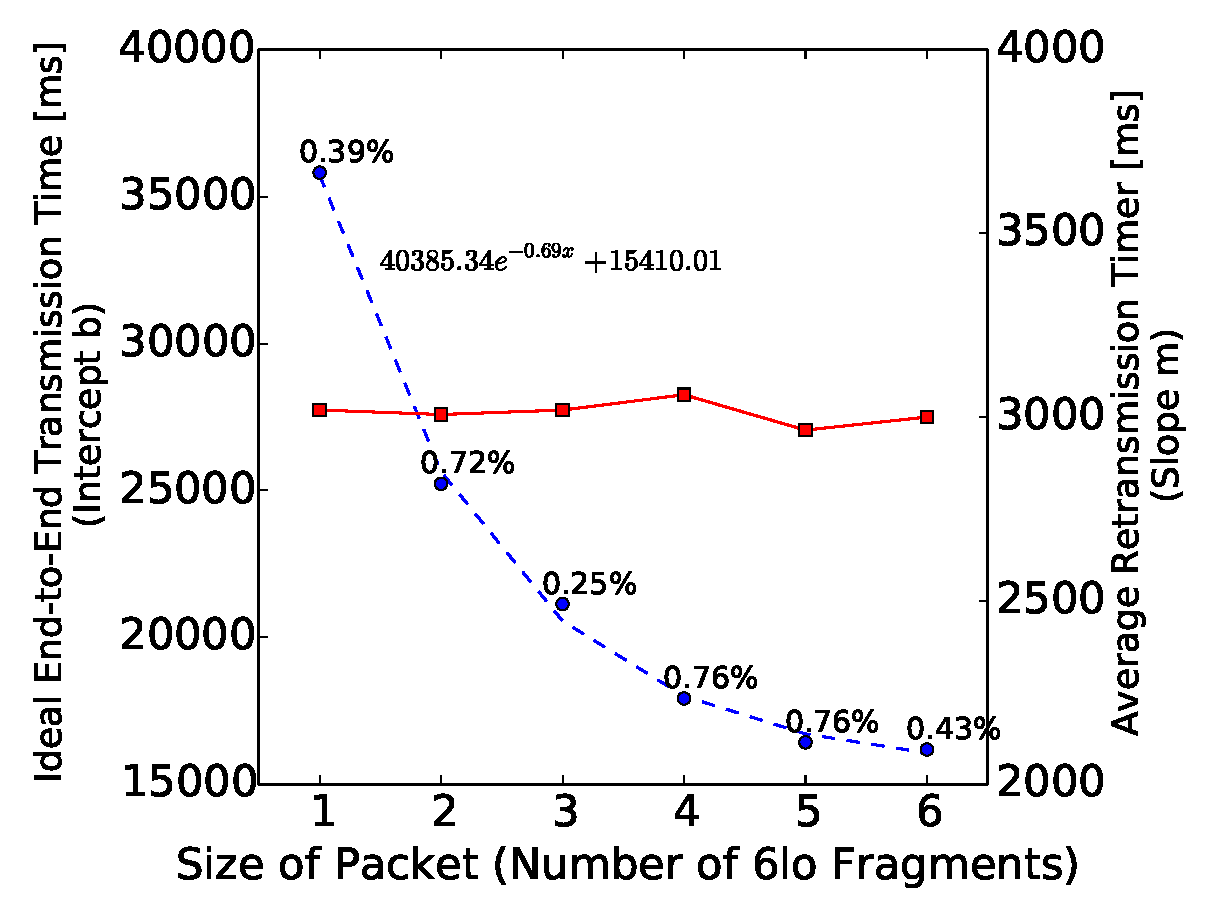
\includegraphics[width=0.5\textwidth]{figs/pa_1}\label{fig:pa1}}
	\subfloat[Linear relationship]{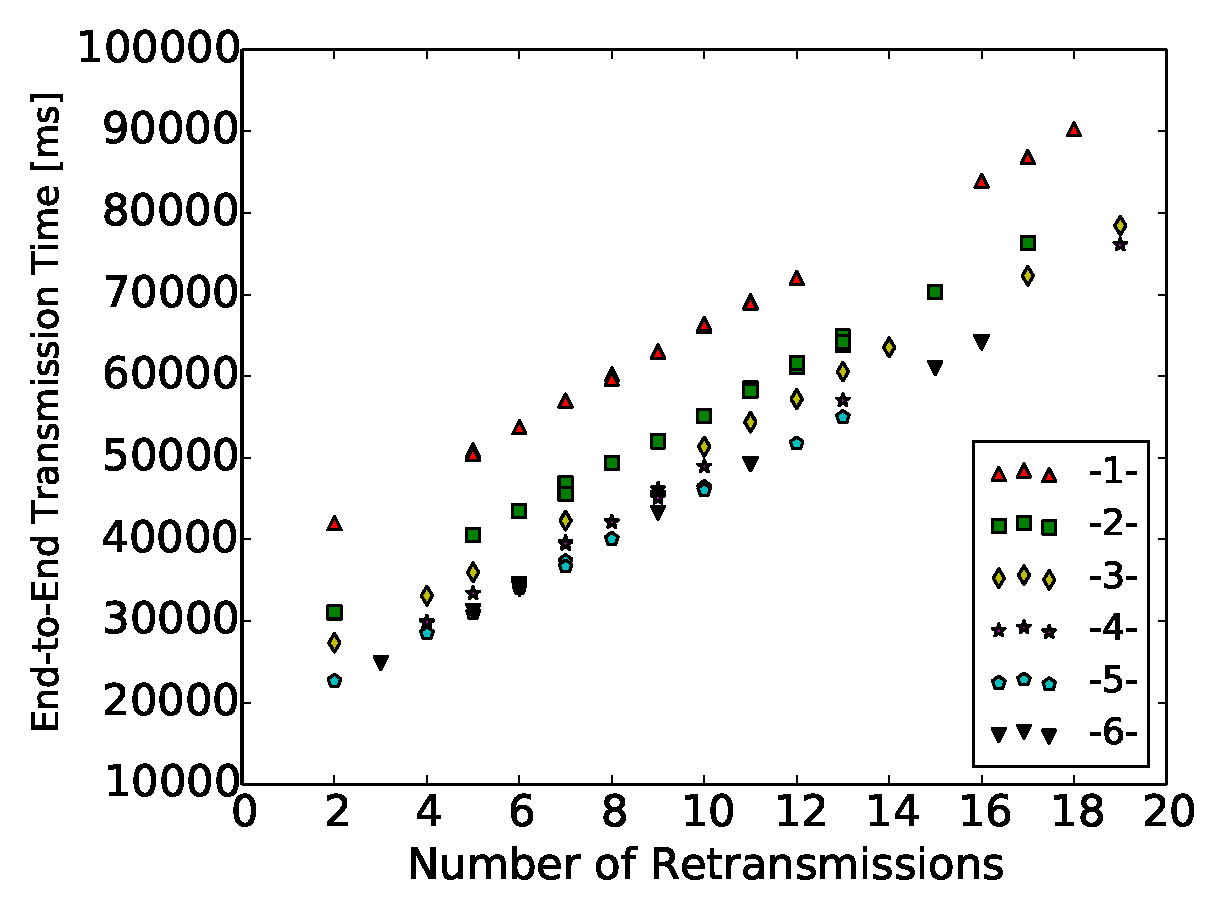
\includegraphics[width=0.5\textwidth]{figs/pa_2}\label{fig:pa2}}
	\caption{Transmitting bulk data (16KiB) in medium traffic (10s) network with link FER(15\%)}
	\label{fig:pa}
	\vspace{-15pt}
\end{figure}

Another function of \emph{Packet Adjustment Module} is to adjust packet size efficiently. When running the experiments in section~\ref{sec:vd}, we find out that there exists a linear relationship between the end-to-end transmission time and the number of retransmissions, as shown in Fig.~\ref{fig:pa2}. For each packet size we use least squares method to fit the scatters by a linear function $y=mx+b$, and the fitted parameters (slope $m$ and intercept $b$) with normalized root-mean-square deviation (NRMSD) are plotted in Fig.~\ref{fig:pa1}. Both $m$ and $b$ have practical meaning: $m$ is the average value of retransmission timer (3 seconds in our experiments); whereas $b$ implies the end-to-end transmission time in ideal situation where no retransmission occurs. From Fig.~\ref{fig:pa1} it is clear to see that intercept $b$ against packet size follows a negative exponential function (dashed line in the figure), which means that the performance gain achievable by increasing packet size is significant when packet size is small; as packet size increases, the gain becomes less significant. With this observation, we set up a threshold value (represented as the number of fragments) in our mechanism. When increasing packet size, if the threshold is not reached, we increase it by one fragment every time; and if the threshold is passed, we increase packet size by its current number of fragments, i.e. doubling the size. Conversely, when decreasing packet size, we half the size if the threshold is not reached; and decrease by one fragment if the threshold is passed.

\section{Evaluation}
We implemented our mechanism on Contiki OS. For the configuration of network stack in Contiki, we chose 6lowpan as the adaptation layer and employed CSMA at the link layer to provide media access control. As applications usually require bulk data to be transmitted as fast as possible, we used maximum power to transmit the data. To minimize the latency caused by wake-up synchronization among nodes, we switched \textit{contikimac} to \textit{nullrdc}, in which nodes do not sleep. In practice, nodes can switch back to \textit{contikimac} after bulk data transmission completes if necessary.

\subsection{Simulation Environment}
We simulated a network containing 20 nodes in Cooja, the standard simulator for Contiki. Each node has a transmission range and a larger interference range. Within transmission range, the frame error rate (FER) is able to be configured and it increases as the transmission distance becomes larger; while in interference range, FER is $100\%$ and other nodes are interfered accordingly. We chose one node as the sender (located at one edge of the network) and another node as the receiver (located at the other edge); there were 4 or 5 hops between the sender and the receiver. Moreover, to increase simulation fidelity, we generated background traffic in the network by making each node (except the sender and the receiver) send small packets to random nodes randomly within an interval. If the interval was set to 0, then no background traffic was generated.

\subsection{Performance through Large Packets} \label{sec:vd}
In section~\ref{sec:ov} we claimed that bulk data transmission in 6lo through large packets can improve network performance significantly. This subsection quantifies this claim. To start with, we consider experiments of medium traffic network (the interval is set to 10 seconds) with different FERs ($0\%$, $15\%$, $30\%$, and $45\%$) where the bulk data (16KiB) are transmitted in different packet sizes. Each experiment was performed 20 times and we use two metrics to compare network performance: end-to-end transmission time, and total transmitted octets by all the nodes along the path from the sender to the receiver. The result from $FER=15\%$ is shown in Fig.~\ref{fig:vd}. Results from other FER values are similar, thus, are omitted for brevity. The exceptional outputs (represented as outliers) are mainly caused by network congestion resulting from the background traffic. Note that the outliers are excluded when calculating the mean value in the figure. Fig.~\ref{fig:vd1} illustrates that as the packet size increases the end-to-end transmission time decreases accordingly; however, when the packet size exceeds a specific value, the transmission time increases again. The same trend occurs for the total transmitted octets, as shown in Fig.~\ref{fig:vd2}. The reasons for this are explained in section~\ref{sec:ov}. From Fig.~\ref{fig:vd}, we can see that if large packets are used, the end-to-end transmission time is improved by $38\%$ (from $\sim 65$s to $\sim 40$s), and total transmitted octets are reduced by $20\%$ (from $\sim 200$KiB to $\sim 160$KiB).
\begin{figure}
	\vspace{-15pt}
	\centering
	\subfloat[End-to-end transmission time (ms)]{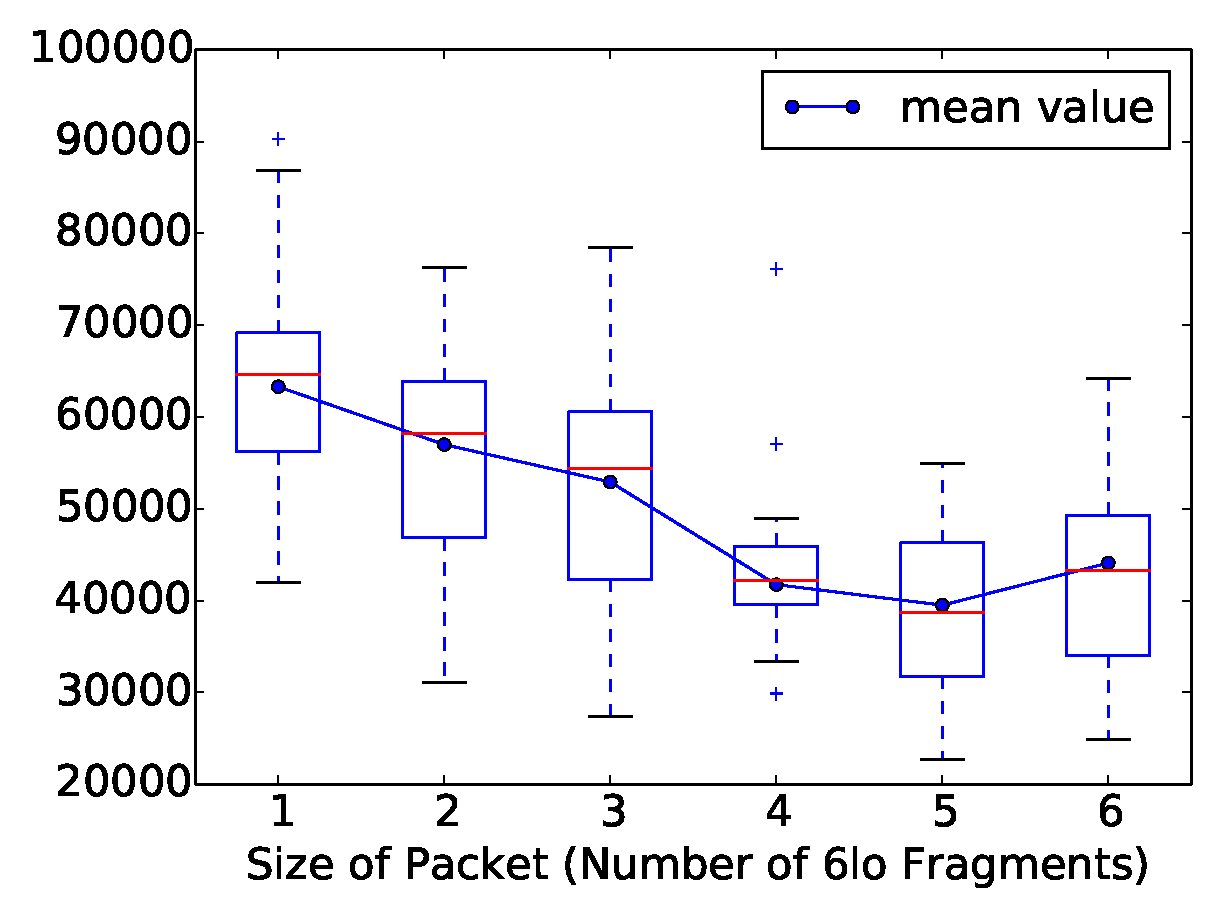
\includegraphics[width=0.5\textwidth]{figs/e2etime}\label{fig:vd1}}
	\subfloat[Total transmitted octets]{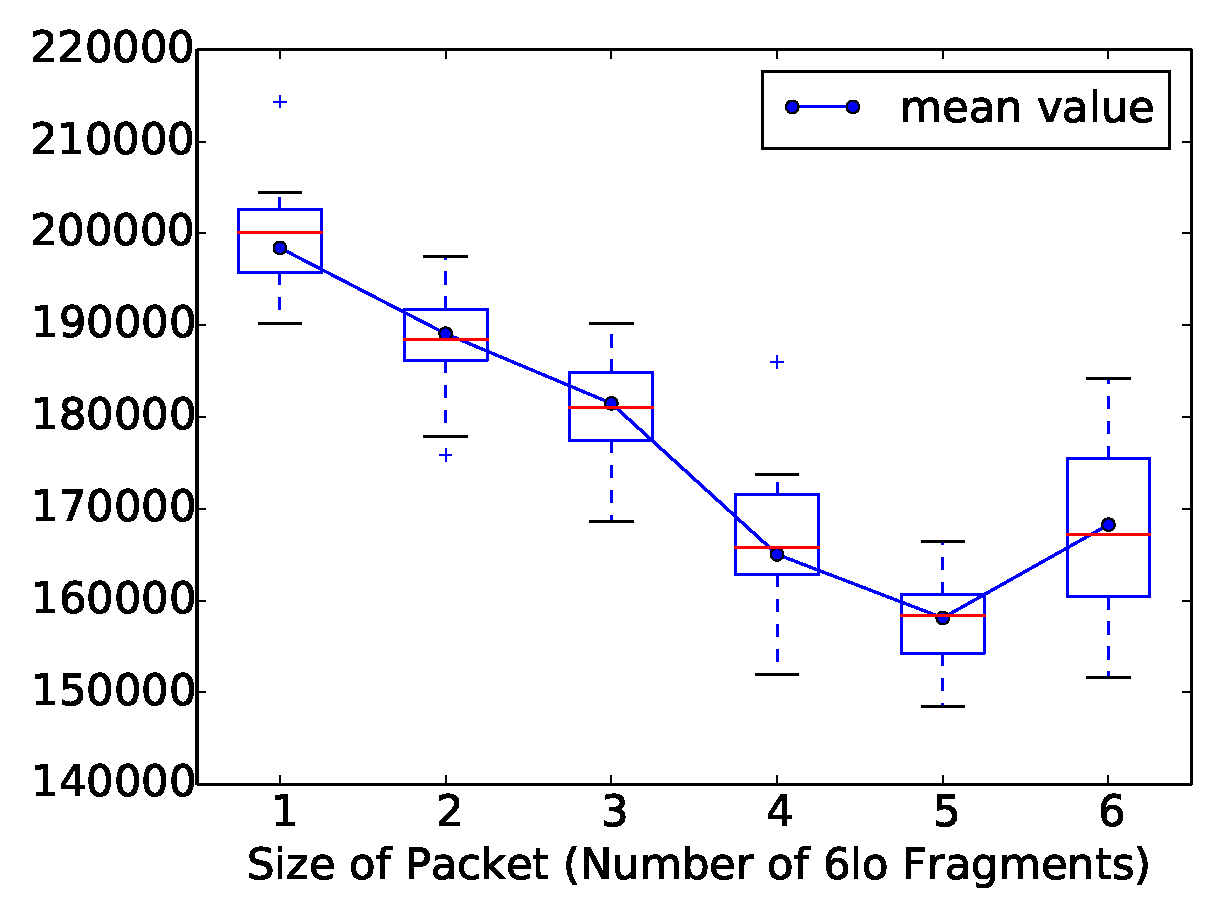
\includegraphics[width=0.5\textwidth]{figs/octets}\label{fig:vd2}}
	\caption{Network performance with $FER=15\%$  for different sizes of packet (represented by number of fragments)}
	\label{fig:vd}
	\vspace{-15pt}
\end{figure}

\subsection{Mechanism Effectiveness}
To evaluate the effectiveness of our adaptive mechanism in terms of reliability and goodput, we investigate a series of experiments similar to those in section~\ref{sec:vd} except two more types of background traffic are introduced: low traffic (the interval is set to 0) and high traffic (the interval is set to 5 seconds). Instead of calculating PLR continuously (cf. section~\ref{sec:ov}) to determine network conditions, we simply define network conditions as bad (if retransmission occurs) or good (if the payload is successfully acknowledged). The threshold value introduced in section~\ref{sec:pa} is set to 3, which means that the possible number of fragments is 1, 2, 3, or 6. Again, each experiment was performed 20 times.

\begin{figure}
	\vspace{-15pt}
	\centering
	\subfloat[Low traffic]{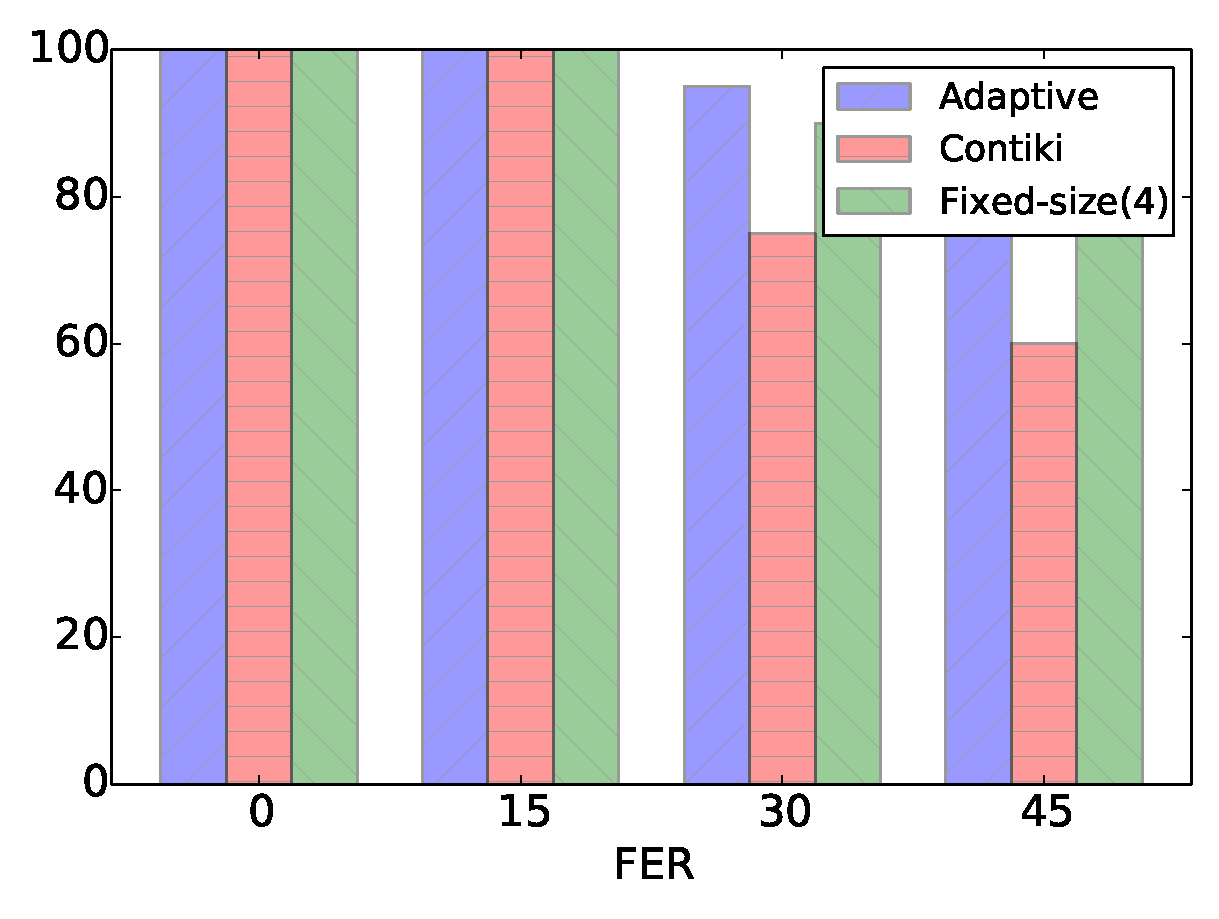
\includegraphics[width=0.33\textwidth]{figs/pct_l}}
	\subfloat[Medium traffic]{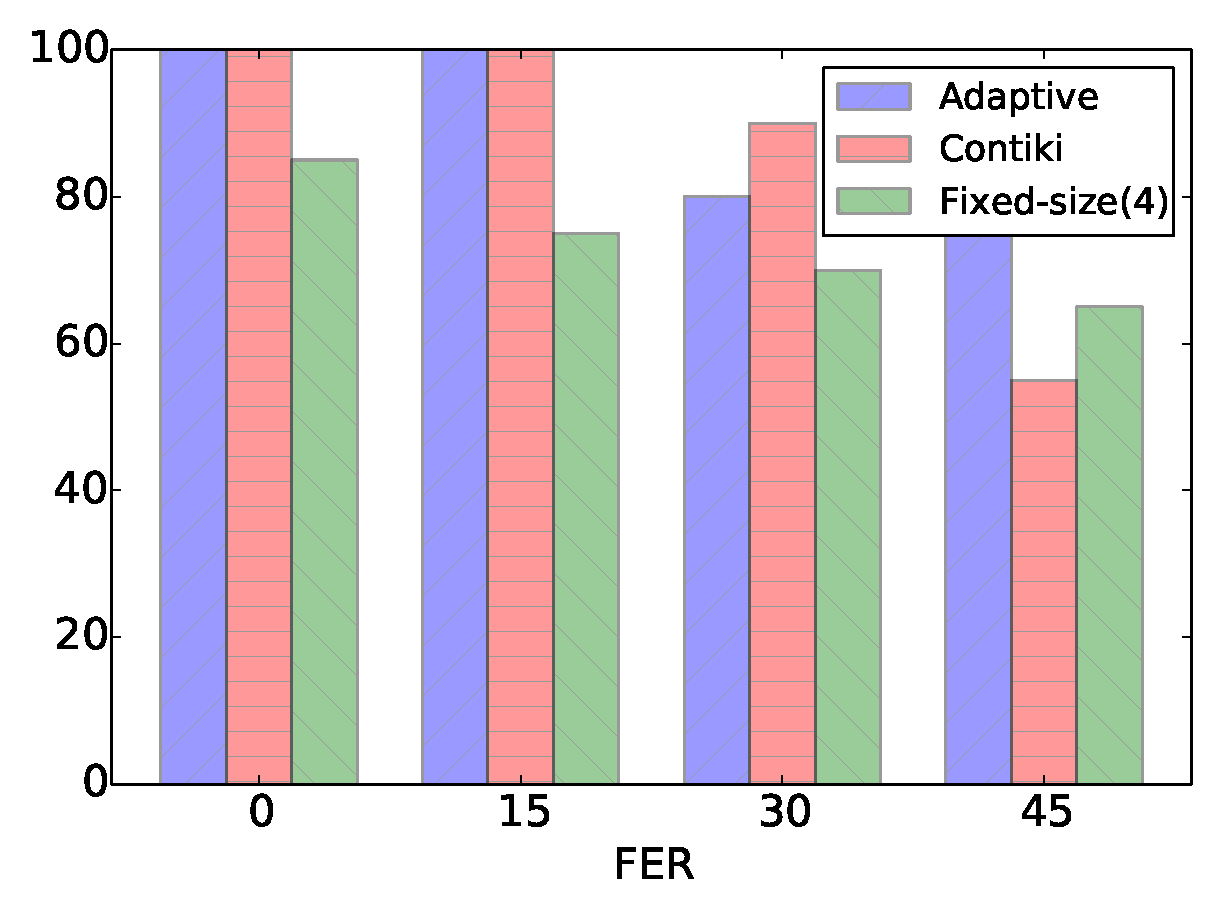
\includegraphics[width=0.33\textwidth]{figs/pct_m}}
	\subfloat[High traffic]{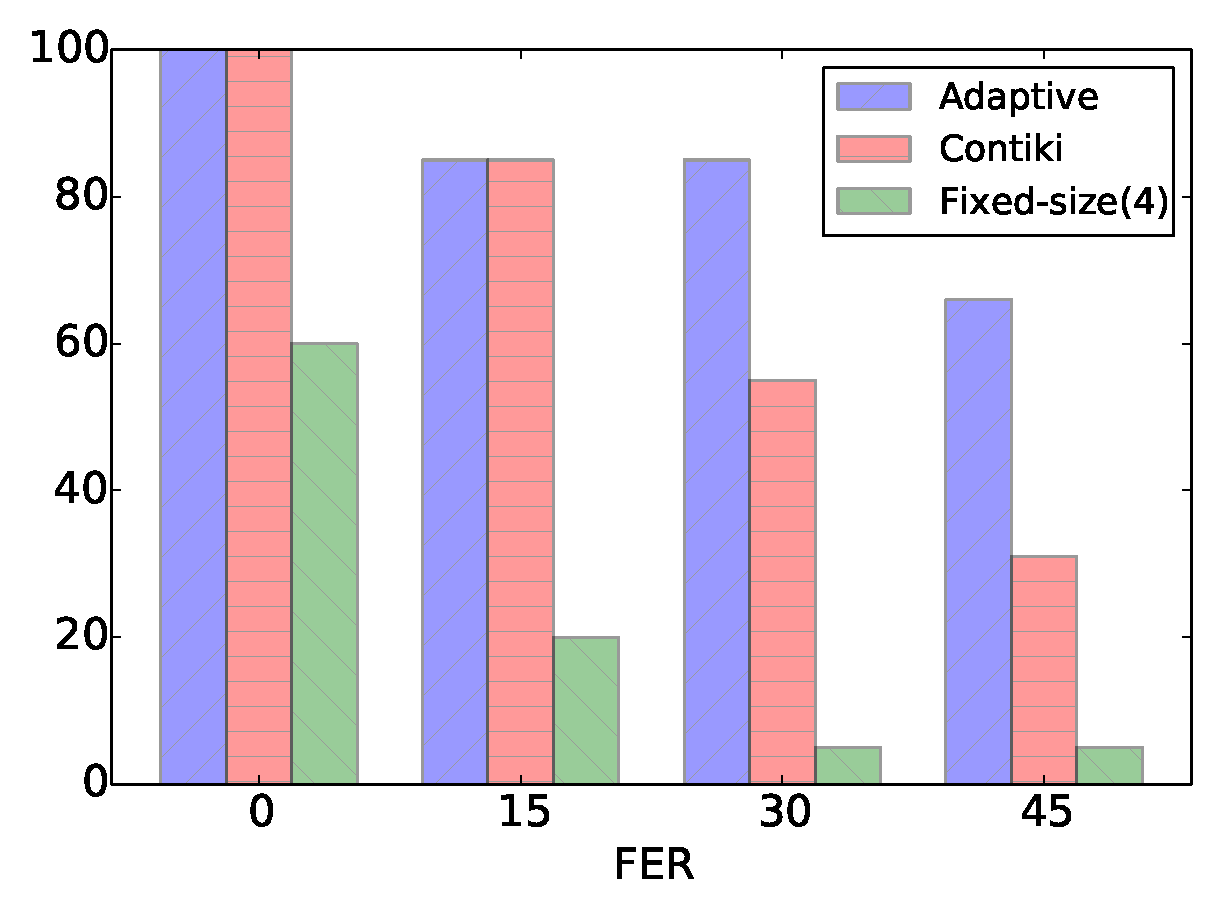
\includegraphics[width=0.33\textwidth]{figs/pct_h}}
	\caption{Percentage of successful transmissions [$\%$], the higher the better.}
	\label{fig:pct}
	\vspace{-15pt}
\end{figure}

We compare our adaptive mechanism (referred to as Adaptive) with the Contiki standard implementation (referred to as Contiki), as well as the approach using a fixed-size packet (referred to as Fixed-size). Firstly, we focus on the percentage of successful transmissions (i.e. how many tests are completed successfully within the 20 tests), which is an indicator of reliability and robustness. The results are shown in Fig.~\ref{fig:pct}. From the figure, we can see that when network traffic is low and link condition is good, all of the three mechanisms complete $100\%$ of tests. When network traffic increases or link condition becomes worse, the percentage of both Adaptive and Contiki decrease slightly, while Fixed-size drops dramatically. We have discussed the reasons for this behaviour in section~\ref{sec:ov}. It is worth mentioning that even in high network traffic with the worst link condition, Adaptive can still complete around $70\%$ of tests, which is significantly higher than that of Contiki. The reason is that the \emph{Unit Discovery Module} in our mechanism ensures that in the worst cases there is no 6lo fragmentation invoked at any node along the path; while in Contiki, intermediate nodes are still possible to trigger 6lo fragmentation that might lead to packet loss in bad network conditions.

\begin{figure}
	\vspace{-15pt}
	\centering
	\subfloat[Low traffic]{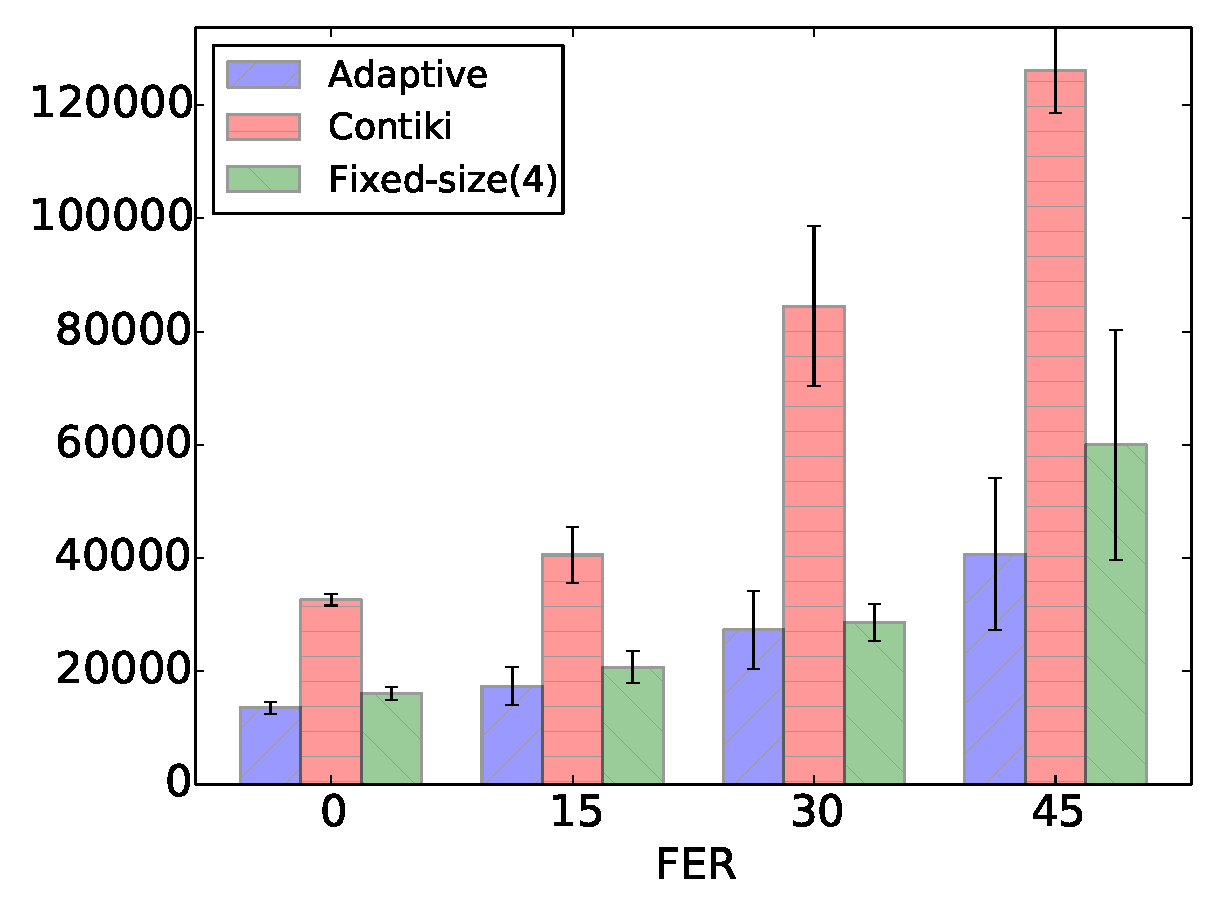
\includegraphics[width=0.33\textwidth]{figs/tm_l}}
	\subfloat[Medium traffic]{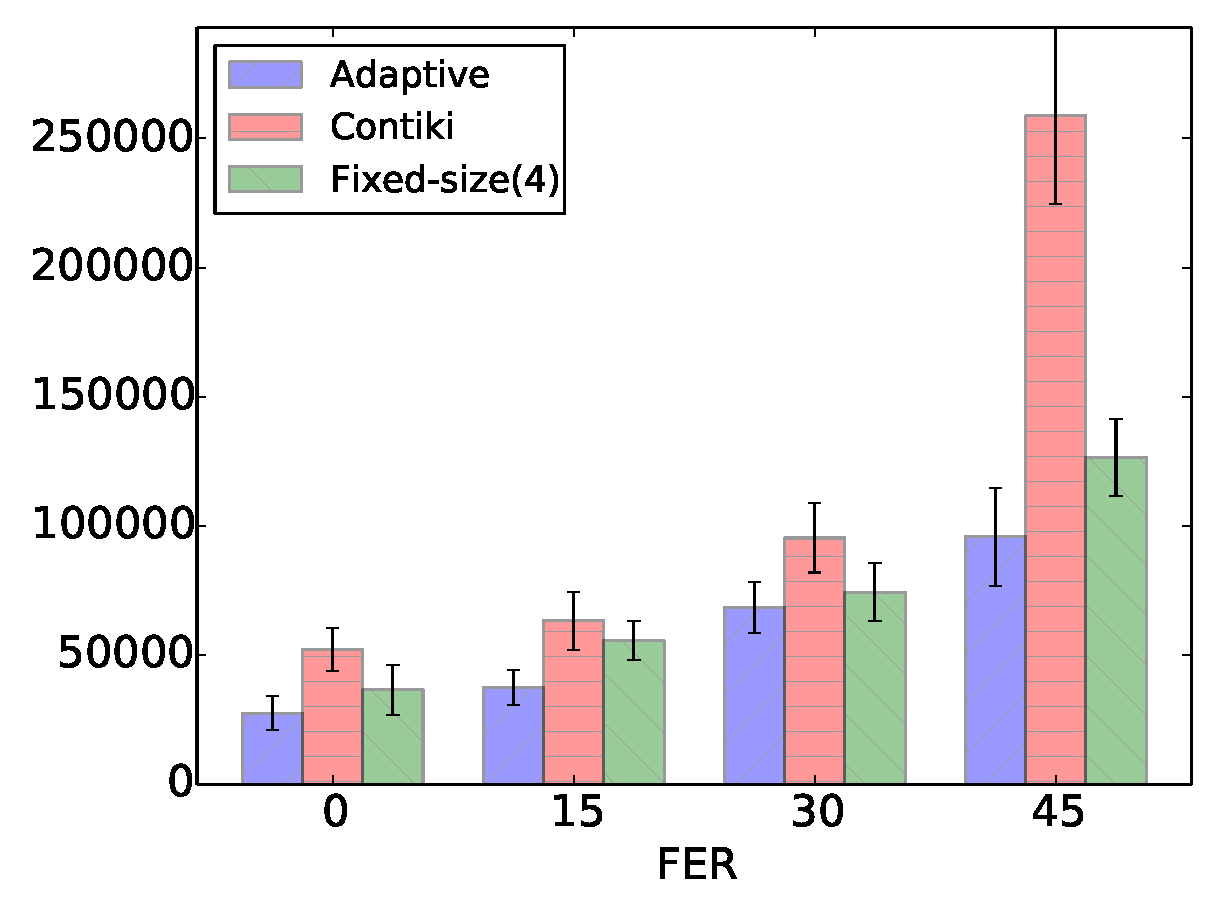
\includegraphics[width=0.33\textwidth]{figs/tm_m}}
	\subfloat[High traffic]{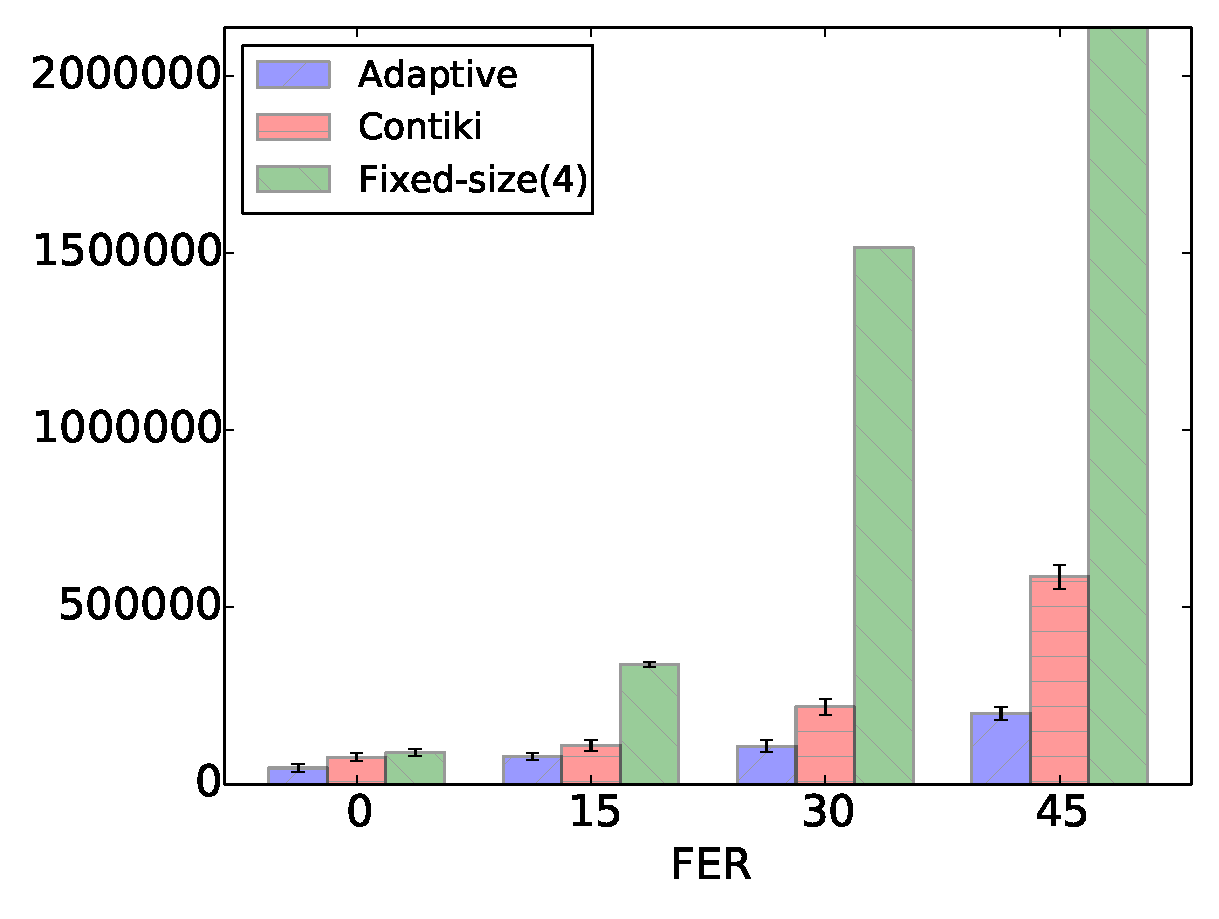
\includegraphics[width=0.33\textwidth]{figs/tm_h}}
	\caption{Estimated end-to-end transmission time [ms], the less the better.}
	\label{fig:tm}
	\vspace{-15pt}
\end{figure}

Secondly, we evaluate network goodput using end-to-end transmission time because network goodput is inversely proportional to end-to-end transmission time. Note that if the test gets failed, it is not possible to acquire the output data. Thus, it is unfair to compare only successful results and exclude the failed cases. To make up for this, we introduce a penalty function, which is defined as $1/percentage$. We then compute the estimated results by successful results times penalty function. We present the estimated results in Fig.~\ref{fig:tm}. From the figure, it is clear that regardless of network traffic, overall transmission time for the three mechanisms increases as link conditions get worse. Compared with Contiki and Fixed-size, Adaptive outperforms them in all three network traffic environments. It is also worth noting that despite the decent performance of Fixed-size for low and medium traffic, the transmission time of it for high traffic is extremely high, which demonstrates its severe weakness in such environments. In summary, our adaptive mechanism is able to provide better reliability and higher goodput than the current state-of-the-art approaches in various network conditions.

\section{Conclusion}
In this paper, we justified the momentum of adjusting packet size adaptively for bulk data transmission in 6lo. Through an empirical study, we made two important observations that inspired the adaptive mechanism design. By evaluating a series of carefully-designed experiments in Cooja, we demonstrated the effectiveness of our mechanism from both reliability and goodput. In the future, we will conduct a systematic study on real devices. Furthermore, power consumption and duty cycles will also be investigated.

\bibliography{bibtex}
\bibliographystyle{plain}
\end{document}